\section{Pattern formation in the Gray-Scott System}
One of the main reasons for the great interest in the Gray-Scott model is its ability to develop complex spatio-temporal patterns. Pattern formation is a form of self-organization which plays a central role in a variety of processes observed in nature that are crucial for the existence of live in any form (see chapter \ref{ch:intro} for examples). In this section it is shown how the developed stochastic simulator can be used to illustrate the temporal evolution of the system. 

The following initial conditions for the number of particles of species U and V are used throughout the whole thesis:
\begin{align}
 u_0 =
  \begin{cases} 
      \hfill    \Omega \left( \frac{1}{2} + \xi\cdot 10^{-2} \right) \hfill & \text{ if $\mathcal{G}_{int}$} \\
      \hfill \Omega \left( 1 + \xi \cdot 10^{-2} \right) \hfill & \text{ otherwise} \\
  \end{cases}
\end{align}
and
\begin{align}
 v_0 =
  \begin{cases} 
      \hfill    \Omega \left( \frac{1}{4} + \xi\cdot 10^{-2} \right) \hfill & \text{ if $\mathcal{G}_{int}$} \\
      \hfill \Omega \left( \xi \cdot 10^{-2} \right) \hfill & \text{ otherwise} \\
  \end{cases}
\end{align}
with random variable $\xi\! \sim\! \operatorname{Unif}(0,1)$ and inner region $\mathcal{G}_{int} = [1/4, 3/4]^d$ where $d$ is the dimension of the system under consideration. The initial conditions were chosen in dependence on \ref{rossinelli_accelerated_2008}. The parameters used are $F=0.04$, $\kappa = 0.06$, $\rho_d = 1-0$ (i.e.\ $\rho_s = 2.0$), $D_u = 2\cdot 10^{-4}$. 

Figure \ref{fig:pattern} illustrates the influence of the scaling parameter $\Omega$. For large values (e.g.\ $\Omega \gtrsim 10000$), the system is close to the thermodynamic limit, i.e.\ the deterministic approach is a valid approximation to the stochastic microscopic phenomena \ref{gillespie_deterministic_2009}. Figure \ref{todo} gives insight into the temporal evolution of the system, figure \ref{fig:3d} shows the isosurface for the concentration of species U at time $t=1000$ with respect to an isovalue of $0.5$. 

\begin{figure}
\centering
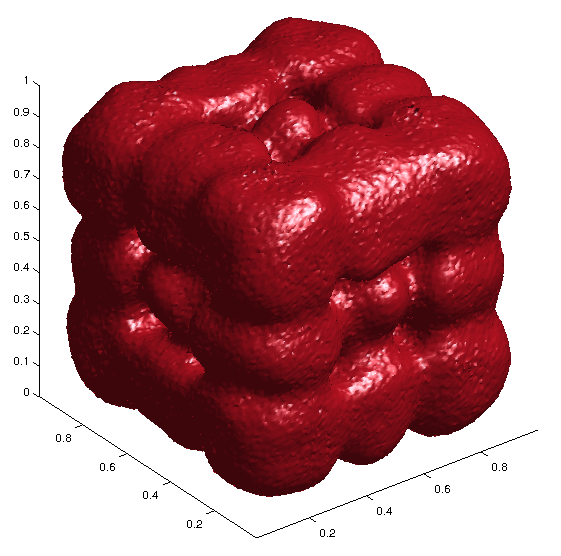
\includegraphics[height=0.4\paperheight]{images/3d.png}
\caption{Isosurface representation of the concentration of species U at $t=1000$ for an isovalue of 0.5.}
\label{fig:3d}
\end{figure}

In the literature and on the Internet numerous articles and websites on Gray-Scott pattern formation exist. Two especially illustrative resources on the topic shall be mentioned here: Project \textit{Xmorphia}\footnote{Original website unavailable. Extended version by R. Munafo: \url{http://goo.gl/vFnOU8}} by Roy Williams at Caltech and the \textit{Amorphous Computing}\footnote{\url{http://goo.gl/4iZUb1}} project by Abelson et al.\ at MIT CSAIL. Both websites enable interactive exploration of the system behaviour under different conditions. The former resource includes a map of the parameter space which directly links to videos that visualize the temporal evolution of the system for the selected setup. The latter includes interactive simulators and videos that illustrate the great variety of patterns that can be obtained. 

%Figure temporal evolution like previous

\begin{figure}
\centering
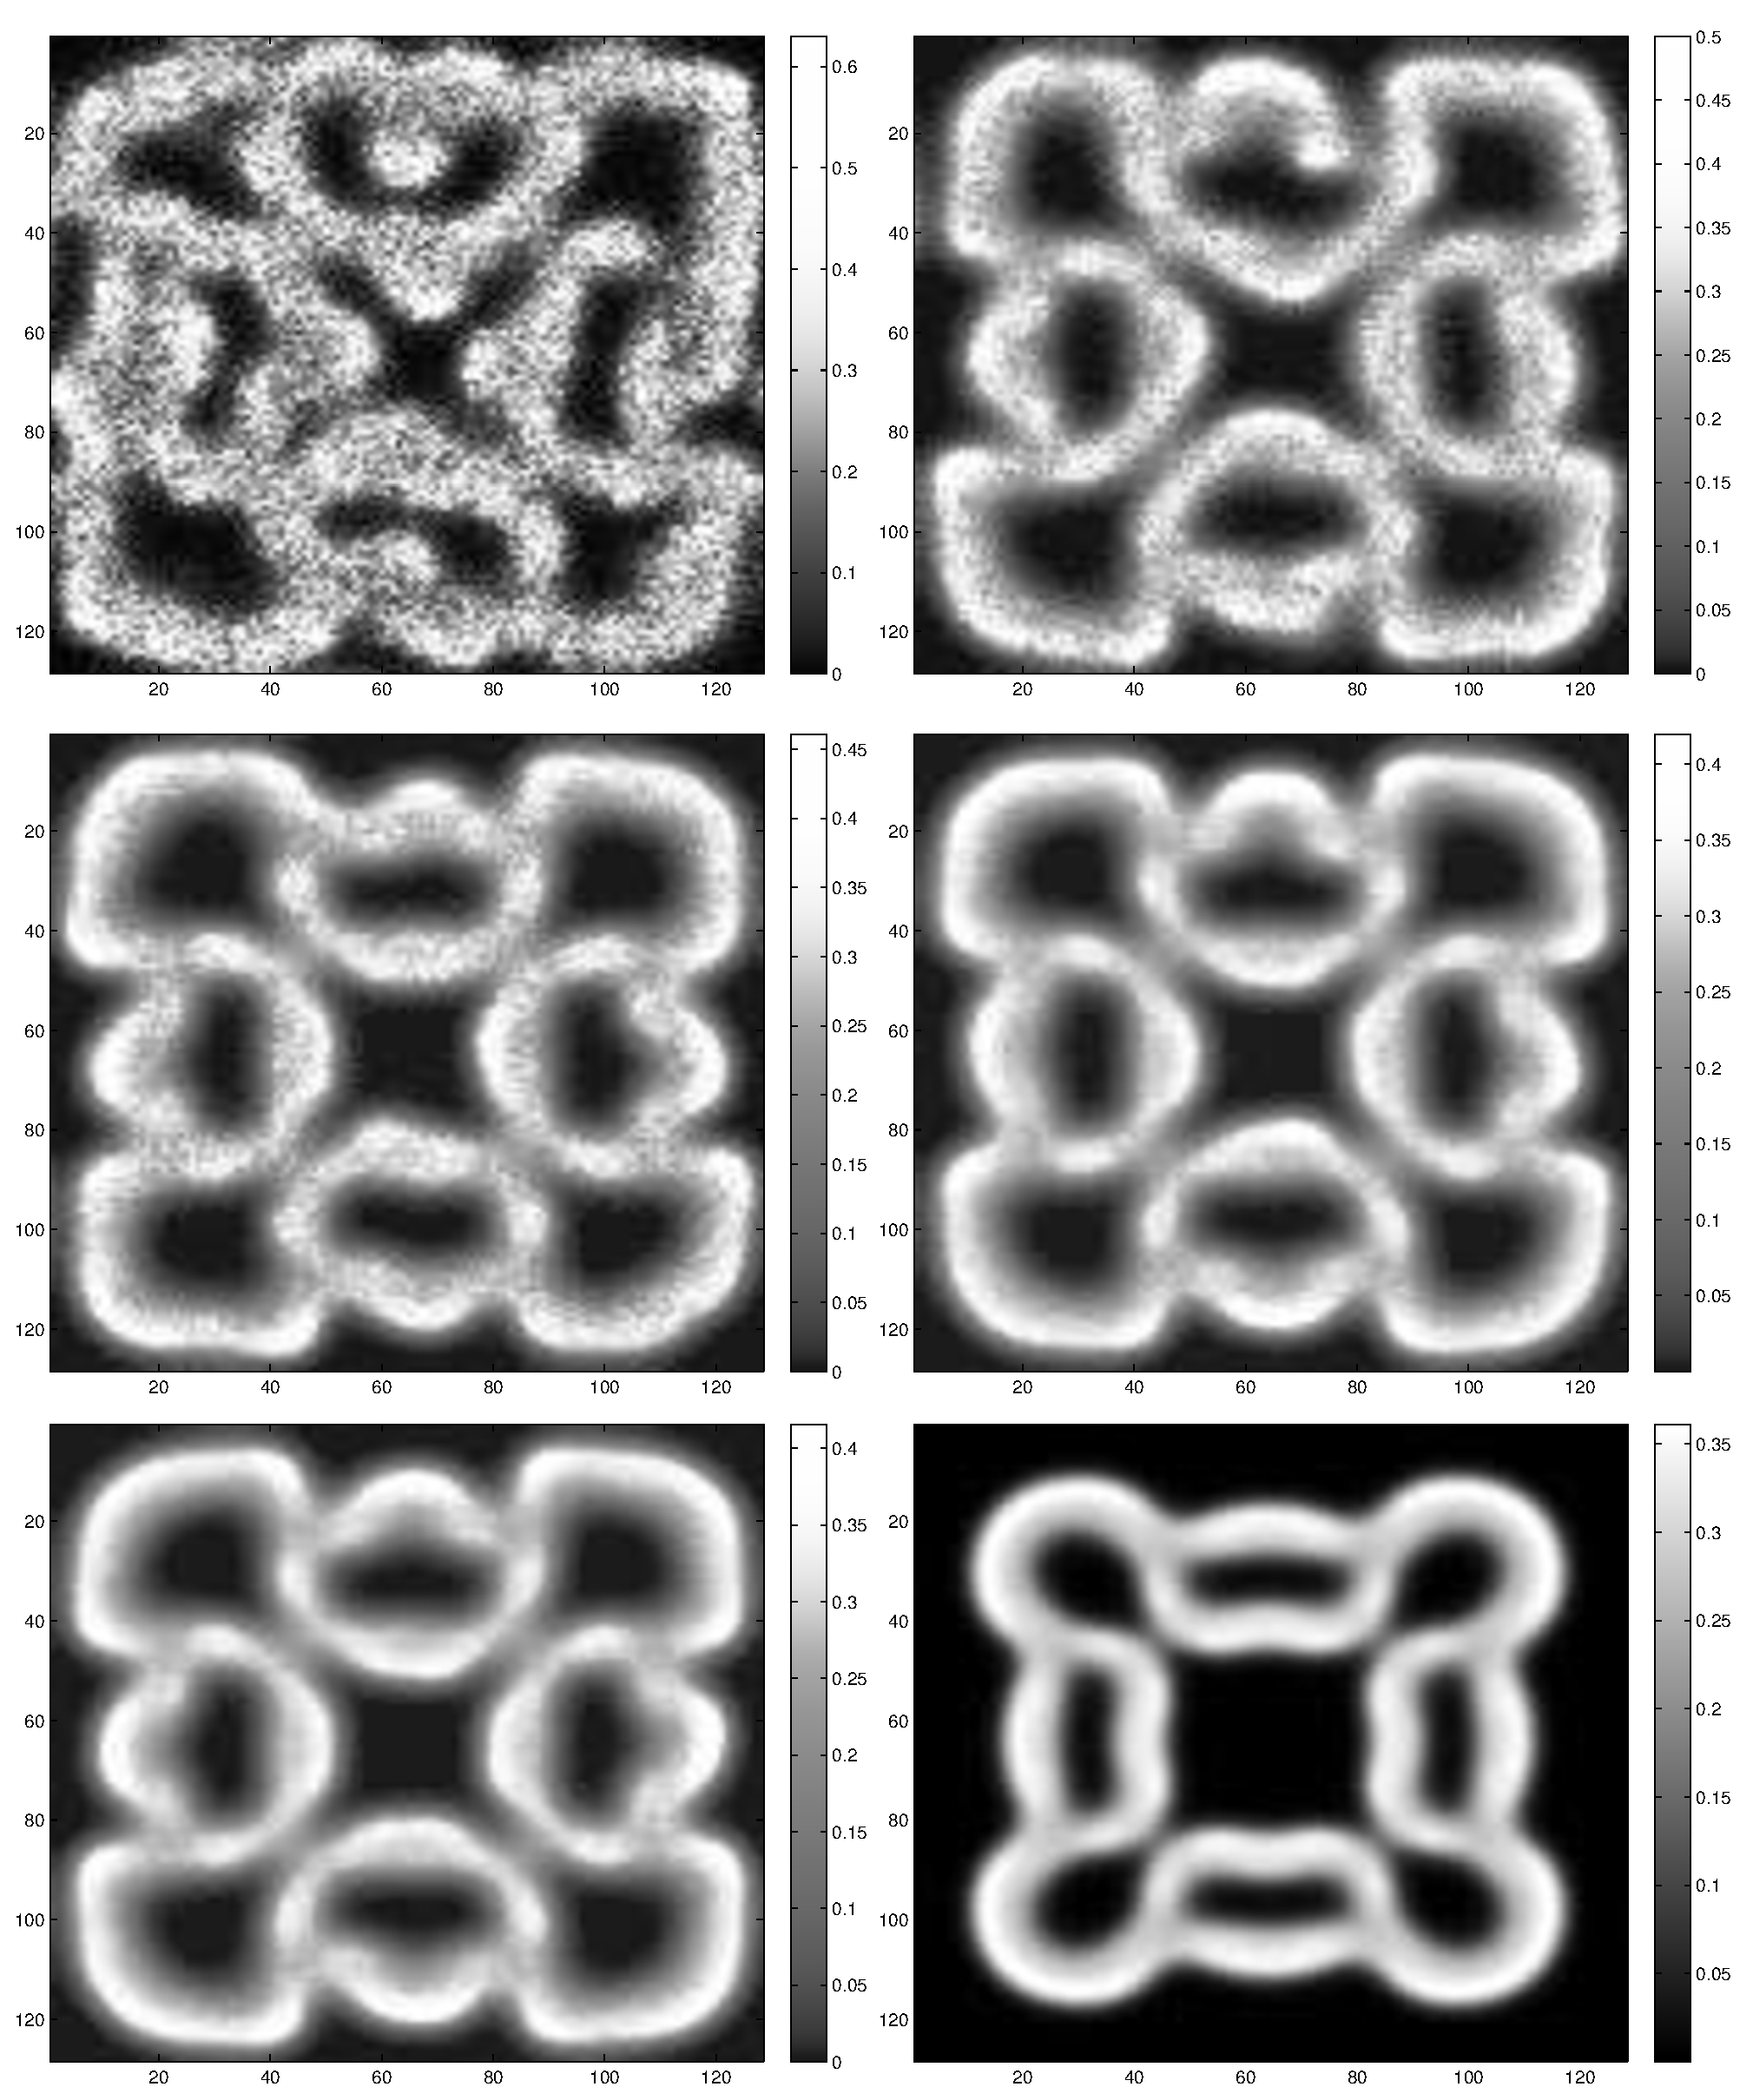
\includegraphics[width=\textwidth]{images/pattern.eps}
\caption{Pattern formation under the influence of varying molecule numbers. Figure shows simulation domain $[0,1]^3$ at time $t=1000$ divided in $128^3$ compartments and sliced at $x=0.6$. Parameters $F=0.04$, $\kappa = 0.06$, $\rho_d = 1-0$ (i.e.\ $\rho_s = 2.0$), $D_u = 2\cdot 10^{-4}$ and $D_v = 1\cdot 10^{-5}$ are used. From left to right and top to bottom the following values for $\Omega$ are used: 100, 500, 1000, 5000, 10000. The plot in the bottom right corner shows the deterministic solution (subject to finite-amplitude random perturbation) obtained with a finite difference approximation. Accuracy control parameter: $\epsilon = 0.05$}
\label{fig:pattern}
\end{figure}